\chapter{Formalism \& numerical methods}

Despite the deuteron problem was solved long time ago, I will describe it briefly 
in order to introduce the notation and formalism. For 3N case only 
extension will be needed.

In order to calculate any observable for the deuteron photodisintegration,
one has to find a nuclear matrix elements:

\begin{equation}
    N^\mu = \langle \Psi_f \vec{P_f} \mid \frac{1}{e}J^\mu(0) \mid \Psi_i \vec{P_i} \rangle =
    \langle p' (l's')j'm_j't'm_t' \vec{P_f} \mid J^\mu \mid \phi_d m_d \vec{P}_i \rangle, 
    \label{main}
\end{equation}
where $J^\mu$ is a four-vector current operator which acts between initial and final 
two-nucleon states. 

% $\vec{P_i}$($\vec{P_f}$) is an initial (final) total 2N m\vec{p}omentum.

% One can introduce relative and total momenta for 2 nucleons:

% \begin{eqnarray}
    %     \vec{p} &=& \frac{1}{2} (\vec{p}_1 - \vec{p}_2)\\
    %     \vec{\mathcal{P}} &=& \vec{p}_1 + \vec{p}_2\\
    %     \pvec{p} &=& \frac{1}{2} (\pvec{p}_1^\prime - \pvec{p}_2^\prime)\\
    %     \pvec{\mathcal{P}}^\prime &=& \pvec{p}_1^\prime + \pvec{p}_2^\prime,
    % \end{eqnarray}
    % where $\vec{p}_1$($\pvec{p}_1^\prime$) and $\vec{p}_2$($\pvec{p}_2^\prime$) are
    % initial(final) momenta of the first and second nucleons.
\section{Deuteron bound state}
    \label{sec:deut_bound}

    Let's find a deuteron bound state wave function $\phi_d$. The time-independent Schr\"{o}dinger
    equation for two particles in such case will be:

    \begin{equation}
        (H_0 + V) \mid \psi_{12} \rangle  = E_d \mid \psi_{12} \rangle,
        \label{shrod_bound}
    \end{equation}
    with a kinetic energy $H_0$ and potential $V$. 
    The kinetic energy $H_0$ can be represented in terms of  relative and total momenta
    of the particles:

    \begin{equation}
        H_0 = \frac{\vec{p}_1^2}{2m_1} + \frac{\vec{p}_2^2}{2m_2} = 
        \frac{\vec{p}^2}{2\mu} + \frac{\vec{\mathcal{P}}^2}{2M}, 
    \end{equation}
    where relative and total momenta are defined as follows:

    \begin{eqnarray}
        \vec{p} &=& \frac{(m_1\vec{p}_1 - m_2\vec{p}_2)}{m_1 + m_2}\\
        \vec{\mathcal{P}} &=& \vec{p}_1 + \vec{p}_2
    \end{eqnarray}
    and $M = m_1 + m_2$ is a total mass, $\mu = \frac{m_1m_2}{M}$ is a relative mass of two nucleons, 
    $\vec{p_i}$ is a momentum of i-th particle.

    Potential $V$ is assumed to depend on the relative degrees of freedom, so
    \eq{shrod_bound} may be decomposed into two separated equations:

    \begin{eqnarray}
        &\frac{\vec{p}^2}{2\mu} \langle \vec{p} \mid \Psi_{int} \rangle +
        \int d \pvec{p} \langle \vec{p} \mid V \mid \pvec{p} \rangle
        \langle \pvec{p} \mid \Psi_{int} \rangle = 
        (E_d - E_{c.m.})\langle \vec{p} \mid \Psi_{int} \rangle \label{se1}\\
        &\frac{\vec{\mathcal{P}}^2}{2M} \langle \mathcal{P} \mid \Psi_{c.m.} \rangle = 
        E_{c.m.}\langle \mathcal{P} \mid \Psi_{c.m.} \rangle \label{se2},
    \end{eqnarray}
    with $\matrixel{\vec{p},\vec{\mathcal{P}}}{H_0}{\Psi_{12}} = \frac{\vec{p}^2}{2\mu} \braket{\vec{p}}{\Psi_{int}} +
    \frac{\vec{\mathcal{P}}^2}{2M} \braket {\mathcal{P}} {\Psi_{c.m.}} $. So $\Psi_{c.m.}$ is a component 
    of total wave function, which reflects a deuteron as a single object with momentum $\vec{\mathcal{P}}$
    while $\Psi_{int}$ is an internal wave function describing interaction between nucleons.
    Basis state $\ket{\vec{p}}$  obeys a completeness
    equation:

    \begin{equation}
        \int d^3\vec{p} \ket{\vec{p}} \bra{\vec{p}}   = \mathbb{1}
    \end{equation}

    Eq.(\ref{se1}) is basically a Schr\"{o}dinger equation for one particle with mass $\mu$ 
    and Eq.(\ref{se2}) can be regarded as a Schr\"{o}dinger equation for particle with mass $M$ in 
    a free motion. Assuming that deuteron is at rest ($E_{c.m.} = 0$) we can stick 
    to the Eq.(\ref{se1}) only. So that:

    \begin{equation}
        \frac{\vec{p}^2}{2\mu} \langle \vec{p} \mid \Psi_{int} \rangle +
        \int d \pvec{p} \langle \vec{p} \mid V \mid \pvec{p} \rangle
        \langle \pvec{p} \mid \Psi_{int} \rangle = 
        E_d \langle \vec{p} \mid \Psi_{int} \rangle
        \label{shrod_old}
    \end{equation}

    Working in 3 dimensional space  is difficult (especially numerically)
    so i introduce the partial-wave representation (PWD) of the momentum state in the following form:

    \begin{equation}
        \mid \vec{p} \rangle = \mid p \alpha \rangle \equiv \mid p (ls) j m_j \rangle \mid t m_t \rangle,
        \label{pwmain}
    \end{equation}
    where we introduce quantum numbers l, s ,j ,t as orbital angular momentum, total spin,
    total angular momentum and total isospin respectively. $m_j$ and $m_t$ are isospin
    and spin projections.


    Yet one can introduce simpler states than it is in (\ref{pwmain}).
    
    \begin{equation}
        \mid p (ls) j m_j \rangle = \sum_{m_l} c(lsj;m_l, m_j\!-\!m_l, m_j) \mid p l m_l \rangle
        \mid s~m_j\!-\!m_l \rangle
        \label{full_decomp}
    \end{equation}

    Also we can decompose spin and isospin states as follows:

    \begin{equation}
        \mid s m_s \rangle = \sum_{m_1} c(\frac{1}{2}\frac{1}{2}s;m_1, m_s\!-\!m_1, m_s)
        \mid \frac{1}{2} m_1 \rangle
        \mid \frac{1}{2} m_s\!-\!m_1 \rangle
        \label{spin_decomp}
    \end{equation}

    \begin{equation}
        \mid t m_t \rangle = \sum_{\nu_1} c(\frac{1}{2}\frac{1}{2}t;\nu_1, m_t\!-\!\nu_1, m_t)
        \mid \frac{1}{2} \nu_1 \rangle
        \mid \frac{1}{2} m_t\!-\!\nu_1 \rangle
        \label{isospin_decomp}
    \end{equation}

    In Eqs.(\ref{full_decomp}) -(\ref{isospin_decomp}),  $c(...)$ are Clebsh-Gordon coefficients.
    Nucleons are spin $\frac{1}{2}$ particles, and also we treat proton and neutron as 
    the same particle in different 
    isospin states, so that isospin is $\nu_1 = \frac{1}{2}$ for proton and $\nu_1 = -\frac{1}{2}$ for neutron.

    The states $\mid p l m_l \rangle$ from Eq.(\ref{full_decomp}) are orthogonal, so that
    
    \begin{equation}
        \langle p^\prime l^\prime m_l^\prime \mid p l m_l \rangle = 
        \frac{\delta(p - p^\prime)}{p^2} \delta_{ll^\prime}\delta_{m_l m_l^\prime}
    \end{equation}
    and also satisfy the completeness relation:

    \begin{equation}
        \sum_{l=0}^\infty \sum_{m_l=-l}^l \int dp p^2 \mid plm_l \rangle \langle plm_l \mid = \mathbb{1}
    \end{equation}


    These states also fulfill a relation

    \begin{equation}
        \langle \pvec{p} \mid plm_l \rangle = 
        \frac{\delta ( \abs{\pvec{p}} - p)}{p^2} Y _{l m_l}(\hat{p}^\prime),
    \end{equation}
    where $Y _{l m_l}(\hat{p}^\prime)$ is a spherical harmonic and 'hat' means a unit vector in 
    direction of $\vec{p}$:

    \begin{equation}
        \vec{p} \equiv |\vec{p}| \hat{p} \equiv p \hat{p} 
        \label{hat}
    \end{equation}

    Nucleons are fermions so exchanging leads to antisymmetry of the
    wave function. In PWD it leads to the
    requirement which
    can be expressed as:

    \begin{equation}
        (-1)^{l+s+t} = -1
        \label{parity}
    \end{equation}

    Taking into account Eq.(\ref{parity}), one can find only one possible PWD state combination for 
    the deuteron bound state(under ... experimental evidence): 2 coupled channels for l=0,2; s=1; j=1and $t = m_t = 0$. 
    These 2 channels are usually denoted as $^3S_1$ and $^3D_1$ and
    corresponding wave functions are $\phi_0(p)$ and $\phi_2(p)$:
    
    \begin{equation}
        \phi_l(p) = \braket{pl}{\Psi_{int}} = \bra{p(l1)1m_d} \braket{00}{\Psi_{int}}; l=0,2.
        \label{deut_waves}
    \end{equation}

    So with a new basis Eq.(\ref{shrod_old}) takes a form:

    \begin{equation}
        \frac{\vec{p}^2}{2\mu} \phi_l(p) +
        \sum_{l^\prime =0,2} \int d p^\prime p^{\prime 2} 
        \langle plm_l \mid V \mid p^\prime l^\prime m_l^\prime  \rangle
        \phi_{l^\prime}(p) = 
        E_d \phi_l(p),
        \label{integral}
    \end{equation}
    for $l=0,2$. In case one does not have a matrix elements for the potential 
    $\langle plm_l \mid V \mid p^\prime l^\prime m_l^\prime  \rangle$ in analytical form,
    but only values for some grid of points, 
    there is still one complication in the Eq.(\ref{integral}) - integration.
    In order to get rid of the integral I use a Gaussian quadrature 
    method of numerical integration \cite{jacobi1826ueber}.
    It allows to replace an integral by the weighted sum:
        $\int_a^b f(x)dx = \sum_{i=1}^n \omega_i f(x_i)$
    In current work I used 72 points in the interval from $0$ to $50 fm$. 
    Using this method, Eq.(\ref{shrod_old}) becomes  

    
    \begin{equation}
        \frac{\vec{p}^2}{2\mu} \phi_l(p) +
        \sum_{l^\prime =0,2}\sum_{j =0}^N  \omega_j p^{\prime 2}_j \langle p_jlm_l \mid V \mid p^\prime_j l^\prime m_l^\prime  \rangle
        \phi_{l^\prime}(p) = 
        E_d \phi_l(p),
        \label{integral2}
    \end{equation}

    I solve this equation as an eigenvalue problem $M\Psi = E_n \Psi$ and
    in that way
    find simultaneously wave function values and binding energy $E_n$. 
    The binding energy $E_n$ calculated with potentials of different chiral orders 
    is presented on the Fig.~\ref{bind}.

    \begin{figure}[h]
        \begin{center}
            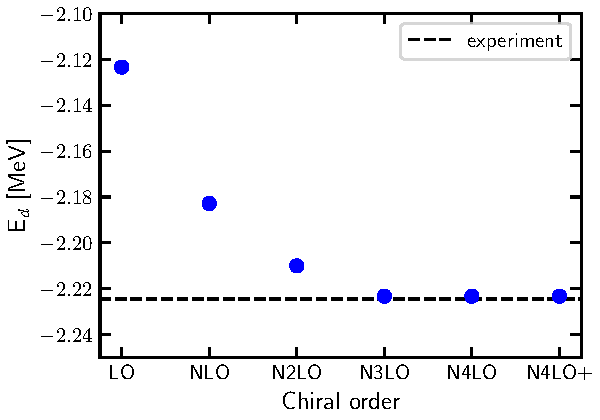
\includegraphics[width=0.65\textwidth]{Figures_python/Binding_energy.pdf}
        \end{center}
        \caption{Deuteron binding energy calculated using chiral potential with different chiral orders.
        Error bands represent a standard deviation of the calculated binding energy with respect to
        the cutoff parameter $\Lambda$.
        Experimental data is taken from \cite{VANDERLEUN1982261}}
        \label{bind}
    \end{figure}

\section{2N scattering state}

\subsection{The Lippmann-Schwinger equation}
    % Let us consider a two-nucleon scattering state $\mid \Psi _f \rangle$, It fulfills
    % a Schr\"{o}dinger equation

    % \begin{equation}
    %     (H_0 + V) \mid \Psi _f \rangle = E \mid \Psi _f \rangle,
    %     \label{schrod_scatt}
    % \end{equation}
    % with $H_0 = \frac{\vec{p}^2}{m}$ and $E > 0$.

    % Solution to the Eq.(\ref{schrod_scatt}) can be presented in the form:

    % \begin{equation}
    %     \mid \Psi _f \rangle = \mid \Psi _0 \rangle + \frac{1}{E - H_0 + i \epsilon} V \mid \Psi _f \rangle
    % \end{equation}

    Let us start from the time-independent formulation of the scattering process.
    In such a case Hamiltonian will be:

    \begin{equation}
        H = H_0 + V,
    \end{equation}
    where $H_0$ is a kinetic energy operator $H_0 = \frac{\vec{p}^2}{2m}$ 
    and $V$ is a nucleon-nucleon interaction.
    For a free particle motion, $V$ will be absent and we will denote an energy eigenstate as
    $\mid \vec{p} \rangle$ - a free particle state.
    In the case of the scattering process, the eigenstate will differ from $\mid \phi \rangle$,
    but in case of elastic scattering (which we re interested in) the energy eigenvalue $E$ should be the same.

    So these two states fulfill Schr\"{o}dinger equations for such scattering process:

    \begin{equation}
        \begin{cases}
            H_0 \mid \vec{p} \rangle &= E \mid \vec{p} \rangle \\
            (H_0 + V) \mid \psi \rangle &= E \mid \psi \rangle
        \end{cases}
        \label{system}
    \end{equation}

    We are interested in solution for Eq.~(\ref{system}), so that 
    $\mid \psi \rangle \rightarrow \mid \vec{p} \rangle$ as $V \rightarrow 0$
    and both $\mid \psi \rangle$ and $\mid \vec{p} \rangle$ have the same energy eigenvalues E.
    As we have scattering process, the energy spectra for both operators $H_0$ and $H_0 + V$
    are continuous. 

    From Eq.~(\ref{system}) follows that

    \begin{equation}
        \mid \psi \rangle = \frac{1}{E - H_0}V \mid \psi \rangle +  \mid \vec{p} \rangle,
        \label{psieq}
    \end{equation}
    where $\mid \vec{p} \rangle$ is a solution to the
    free-particle Schr\"{o}dinger equation
    \begin{equation}
        H_0 \ket{\vec{p}} =  E  \ket{\vec{p}},
    \end{equation}
    with same energy eigenvalue\cite{Sakurai}.
    % was added artificially in order to satisfy a criterion mentioned above 
    % and following the logic from . 
    In addition, it guarantees that
     application of the operator $(E -H_0)$ to the 
    (\ref{psieq}) results in the second equation from the system (\ref{system}).
    % Also, \eq{psieq} for $V \rightarrow 0$ becomes $\mid \psi \rangle = \mid \vec{p} \rangle$


    In order to deal with a singular operator $\frac{1}{E - H_0}$ in eq.(\ref{psieq}), the well-known
    technique is to make such an operator complex by adding small imaginary number to the denominator
    so Eq.(\ref{psieq}) becomes
    % making it  $\frac{1}{E + i\epsilon - H_0}$.

    \begin{equation}
        \ket{\psi} = G_0(E \pm i\epsilon)V \mid \psi \rangle +  \mid \vec{p} \rangle,
        \label{lse}
    \end{equation}
    where $G_0$ is a free propagator:

    \begin{equation}
        G_0(z) = \frac{1}{z - H_0}
        \label{g0}
    \end{equation}

    Solution with $G_0(E - i\epsilon)$ corresponds to the incoming spherical wave,
    while $G_0(E + i\epsilon)$ - to the outgoing one. Since we are interested in the scattering
    process, only the $(+)$ sign survives.
    
    Eq.~(\ref{lse}) is known as a Lippmann-Schwinger equation (LSE) and using
    the definition of the transition operator $t$:

    \begin{equation}
        t \ket{\vec{p}} = V \ket{\psi}
        \label{t-op}
    \end{equation}
    we can rewrite it as 

    \begin{equation}
        \ket{\psi} = (1 + G_0(E + i\epsilon)V t)  \ket {\vec{p}}
        \label{psi_toper}
    \end{equation}

    With substitution of \eq{lse} into \eq{t-op} we can find
    an explicit form of the $t$ operator:

    \begin{eqnarray}
        t \ket{\vec{p}} = V G_0(E + i\epsilon)V \mid \psi \rangle +  V \mid \vec{p} \rangle = \nonumber\\
        = V G_0(E + i\epsilon) t \ket{\vec{p}} +  V \mid \vec{p} \rangle
        \label{top2}
    \end{eqnarray}

    Getting rid of the initial state $\ket{\vec{p}}$ in the \eq{top2} we can get a LSE
    for the transition operator in the iterative form:

    \begin{eqnarray}
        t = V + V G_0V t = \nonumber\\
        = V + V G_0 V + V G_0 V G_0V + ...
    \end{eqnarray}

    In the partial-wave representation, LSE \eq{top2} may be written as:
    \begin{multline}
        \matrixel{p^\prime (l^\prime s^\prime)jt}{t(E)}{p(ls)jt} = 
        \matrixel{p^\prime (l^\prime s)jt}{V}{p(ls)jt} + \\
        +\sum_{l^{\prime\prime}} \int_0^\infty dp^{\prime \prime} p^{\prime \prime 2}
        \matrixel{p^\prime (l^\prime s)jt}{V}{p^{\prime\prime}(l^{\prime\prime} s)jt} \\
        \cross \frac{1}{E + i\epsilon - p^{\prime \prime 2}/m}
        \matrixel{p^{\prime \prime} (l^{\prime \prime} s)jt}{t(E)}{p^{\prime\prime}(l s)jt}
        \label{lse_pwd}
    \end{multline}

    Using \eq{psi_toper} we can write \eq{main} as
    
    \begin{equation}
        N^\mu = \bra{\phi m_p m_n} (1 + G_0(E + i\epsilon)V t) \frac{1}{e}J^\mu(0) \mid \Psi_i \vec{P_i} \rangle
        \label{main_top}
    \end{equation}

    %TODO: rewrite everything in \phi m_d m_n
    
\section{3N bound state}

    The 3N bound state is derived from a general Schr\"{o}dinger for 3N system
    and its total wave function obeys the following equation:

    \begin{equation}
        \ket{\Psi_i} = G_0(E+i\epsilon)\sum_{j=1}^3 (V_j + V_4^j) \ket{\Psi_i},
        \label{psi3_total}
    \end{equation}
    where $G_0$ is a free propagator from \eq{g0}, $V_j$ - is a two-body potential
    acting between nucleons $k$ and $l$ (j, k and l - are the numbers of each nucleon)
    and $V_4^j$ is a component of three-body potential $V_4 = \sum_{j=1}^3 V_4^j$.
    E - is a binding energy.

    \eq{psi3_total} can be split into 3 independent equations for
    so-called Faddeev components $\ket{\psi_j}$

    \begin{equation}
        \ket{\Psi_i} = \sum_{j=1}^3 \ket{\psi_j}.
        \label{faddeev_comps}
    \end{equation}

    Using \eq{faddeev_comps} one can decompose \eq{psi3_total} into 
    separate equations for each Faddeev component:

    \begin{equation}
        \ket{\psi_j} = G_0(E+i\epsilon)(V_j + V_4^j) \ket{\Psi_i},
        \label{psi3_component}
    \end{equation}

    Next I introduce a permutation operator P, which is a combination
    of operators $P_{jk}$:
    
    \begin{equation}
        P = P_{12}P_{23} + P_{13}P_{32}.
        \label{permutation}
    \end{equation}

    The operator component $P_{jk}$ acting on the state interchange the momenta and  
    quantum numbers of the nucleon number $j$ and$k$.

    Using \eq{permutation} and \eq{faddeev_comps},
    one can rewrite \eq{psi3_component} in the following form:

    \begin{equation}
        \ket{\psi_j} = G_0(E+i\epsilon)t_j P \ket{\psi_i} + 
        (1 + G_0(E+i\epsilon)t_j)G_0(E+i\epsilon)V_4^j(1+P)\ket{\psi_i},        
    \end{equation}
    where $t_j$ is a two-body t-operator which obeys \eq{top2} for corresponding 
    two-body potential $V_j$.





\section{Nd scattering state}
\label{nd_state}

    Analogously to the bound state, one can express a nucleon-deuteron
    scattering state
    using a permutation operator \eq{permutation}.

    \begin{equation}
        \ket{\Psi^{(-)}}^{Nd} = \frac{1}{\sqrt{3}}(1+P)\ket{\Psi^{(-)}_1}^{Nd}    
    \end{equation}

    A scattering state $\ket{\Psi^{(-)}_1}^{Nd}$ can be expressed
    in terms of asymptotic state $\ket{\Phi^{Nd}_1}$, where particles
    2 and 3 form a deuteron and the third particle (number 1) is a nucleon
    which propagates freely with relativemomentum $\vec{q}_0$ with 
    respect to the deuteron:

    \begin{eqnarray}
        \ket{\Psi^{(-)}_1}^{Nd} &\equiv& \lim_{\epsilon \rightarrow 0} 
        i \epsilon G(E_{Nd} - i\epsilon)\ket{\Phi^{Nd}_1}\\
        \ket{\Phi^{Nd}_1} &\equiv& \ket{\Phi_{d(2,3)}}\ket{\vec{q}_0},
    \end{eqnarray}
    where $\ket{\Phi_{d(2,3)}}$ is a deuteron wave function and 
    $\ket{\vec{q}_0}$ - a free particle state. $E_{Nd}$
    is a total energy of the 3N system:

    \begin{equation}
        E_{Nd} = E_d + \frac{3 |\vec{q}_0|^2}{4m},
    \end{equation}
    where $E_d$ is a deuteron binding energy and m - nucleon mass. 

    The full propagator $G(E_{Nd})$ in this case takes a form:
    
    \begin{equation}
        G(z)= \frac{1}{z - (H_0 + \sum_{i=1}^4V_i)}
    \end{equation}


\section{3N scattering state}

    As in Sec.~\ref{nd_state}, one can
    write an equation for the 3-nucleone scattering state:

    \begin{equation}
        \ket{\Psi^{(-)}}^{3N} = \frac{1}{\sqrt{3}}\ket{\Psi^{(-)}_j}^{3N}    
    \end{equation}
    with a set of corresponding equations for $\ket{\Psi^{(-)}_j}^{3N}$

    \begin{eqnarray}
        \ket{\Psi^{(-)}_j}^{3N}  &\equiv& \lim_{\epsilon \rightarrow 0}
        i \epsilon G(E_{3N} - i\epsilon)\ket{\Phi^{3N}_j}\\
        \ket{\Phi^{3N}_j} &\equiv& \frac{1}{\sqrt{2}}(1 - P_{kl})
        \ket{\vec{p}(kl)\vec{q}(j)}\\
        E_{3N} &=& \frac{|\vec{p}|^2}{m} + \frac{3 |\vec{q}|^2}{4m},
    \end{eqnarray}


    \section{Nuclear electromagnetic current}

\section{Theoretical uncertainties}
    
    \subsection*{Truncation error}
    \label{sec:trunc}

    As it was mention above, each subsequent order of chiral
    expansion provide us with more and more sophisticated
    potential. Starling from the leading order (LO) and coming to next
    N2LO, N3LO and so on we toke into account more Feynmann diagrams 
    and in result potential is able to provide us with more precise predictions
    for the regarded process and observable. But the chiral expansion (as any expansion) 
    in principle can be continued to the infinity, improving the resulting series.
    In practice we are limited by some number of terms, but we would like to find out
    the uncertainty appearing from cutting off remaining part of the expansion.
    This uncertainty is called a truncation error and there some ways of estimation its value
    for the potential of each order of chiral expansion having predictions for some limited number
    of terms \cite{Epelbaum2015_trunc, Epelbaum2014SCS, Binder2015, Epelbaum_pos}.

    Let's regard some observable $X^i(p)$ which is calculated at $i$-s order of chiral expansion 
    with expansion parameter $Q$ ($i = 0,2,3...)$\footnote{We do not have a first order of expansion
    because this term in chiral expansion is always vanished
    and NLO  corresponds to the quadratic term (number 2)}.
    Here $p$ specifies
    {\textcolor{red}{?????}} a momentum
    scale of the current reaction in the center of mass frame (in the case of deuteron photodisintegration it would be a
    photon's momentum).  

    If I define a difference between observable at each subsequent orders as:

    \begin{equation}
        \Delta X^{(2)} = |X^{(2)} - X^{(0)}|, \Delta X^{(i>2)} = |X^{(i)} - X^{(i-1)}|,
    \end{equation}
    then chiral expansion for X can be written as:

    \begin{equation}
        X = X^{(0)} + \Delta X^{(2)} + \Delta X^{(3)} + ... + \Delta X^{(i)}
        \label{trunc1}
    \end{equation}
        
    The truncation error at order i $\delta X^{(i)}$ is estimated using actual and expected values of the observable at 
    higher orders. In order to do that I use following expressions:

    \begin{eqnarray}
        \delta X^{(0)} &=& Q^2 \left| X^{(0)} \right| \label{trunc2}\\ 
        \delta X^{(i)} &=& \max_{2 \leq j \leq i} \left( Q^{i+1} \left| X^{(0)} \right|,
        Q^{i+1-j} \left| \Delta X^{(j)} \right| \right) \label{trunc3} 
    \end{eqnarray}

    Additionally, following the \cite{Binder2015} I use the actual high-order predictions 
    in order to specify uncertainties so that:

    \begin{equation}
        \delta X^{(i)} \geq \max_{j,k} (|X^{j \geq i} - X^{k \geq i}|)
        \label{trunc4}
    \end{equation}
    and to be conservative I use additional restriction:

    \begin{equation}
        \delta X^{(i)} \geq Q \delta X^{(i-1)}
        \label{trunc5}
    \end{equation}

    
    \begin{figure}[h]
        \begin{center}
            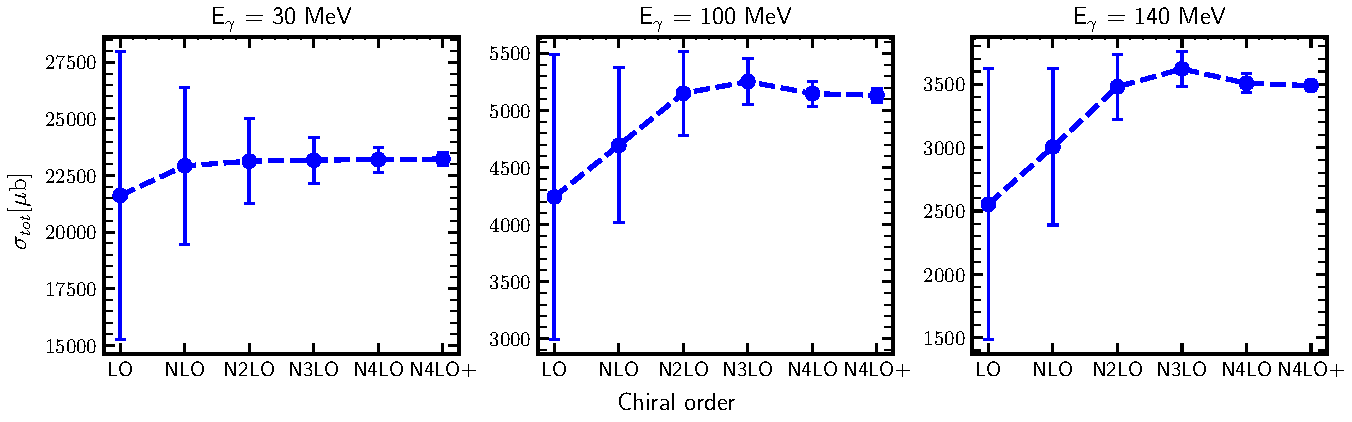
\includegraphics[width=0.95\textwidth]{Figures_python/TOTAL_CROSSSECTION_Truncation.pdf}
        \end{center}
        \caption{Total cross section of the deuteron photonisintegration
        process as a dependance on the chiral order for three photon energy E$_\gamma$ values: 30, 100 and 140 MeV.
        Error bands show an estimated truncation error at each order.}
        \label{Trunc_100}
    \end{figure}
    
    In Fig. \ref{Trunc_100} I present a total cross-section for the deuteron photodisintegration 
    at 3 photon energie values: 30,100 and140 MeV as a dependance on the chiral order.
    Error bands show truncation errors calculated using described above method.
    One can see that errors are being reduced with each consecutive chiral order: for LO it is the biggest
    while for N4LO+ it is hardly visible at presented scale.


    \subsection*{Cutoff dependency}



    Another uncertainty comes from the choice of the cutoff parameter's value 
    which was mentioned already.

   According to \cite{reinkrebs2018}, where the SMS potential was presented,
   4 values of the cutoff parameter $\Lambda$ are recommended: 400, 450, 500 and 550 MeV.
   Using each of them one obtains different predictions which may differ 
   from actual (experimental) value. Therefore the choice of $\Lambda$ value
   may affect a quality of the prediction.


   \begin{figure}[h]
    \begin{center}
        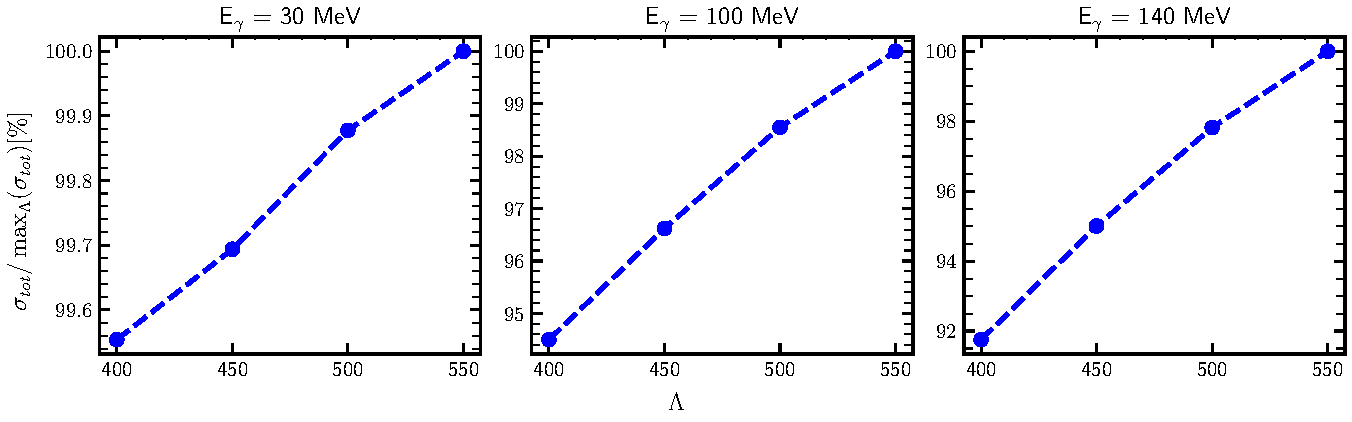
\includegraphics[width=0.95\textwidth]{Figures_python/TOTAL_CROSSSECTION_cutoff.pdf}
    \end{center}
    \caption{Total cross section of the deuteron photonisintegration
    process as a dependance on the cutoff parameter $\Lambda$ 
    for three photon energy E$_\gamma$ values: 30, 100 and 140 MeV.}
    \label{Cutoff_dep}
    \end{figure}

    The comparison of predictions obtained with different values of the 
    cutoff parameter $\Lambda$ is presented on the Fig.~\ref{Cutoff_dep}.
    Each subfigure shows a predictions for the total cross section as 
    a function of the cutoff parameter for the photons energies 30, 100 and 140~MeV
    normalized be the maximum value among all $\Lambda$ 
    (at the chiral order N$^4$LO+).
    As we can see,
    there is almost linear dependance with positive linearity coefficient value:
    with higher $\Lambda$ the cross section value increases as well.
    The noticeable is also the fact, that with higher photon's energy,
    the cutoff dependance becomes stronger: fro $E_\gamma=30$~MeV
    the maximal difference between predictions is around 0.5\% while
    for 140~MeV it increases to more than 8\%. This results are
    generally within our beliefs that our model works better for
    smaller energies. 






















    % Let me move to the coordinate representation of the Eq.~(\ref{lse}):

    % \begin{equation}
    % \langle \vec{x}  \mid \psi \rangle = \langle \vec{x}  \mid \frac{1}{E + i\epsilon - H_0}V \mid \psi \rangle + \langle \vec{x}  \mid \vec{p} \rangle
    % \label{lse_coord}
    % \end{equation}

    % If we choose $\ket*{\vec{x}}$ to be normalized as
    % $\braket{\vec{x}^\prime}{\vec{x}} = \delta^3(\vec{x}^\prime - \vec{x})$ ,
    % the Fourier transform will give us \cite{elster_lectures}: 
    % \begin{equation}
    %     \braket{\vec{x}}{\vec{p}} = \frac{1}{(2 \pi)^{3/2}} e^{i \vec{p} \cdot \vec{x}}.
    %     \label{planewave}
    % \end{equation}

    % I can rewrite Eq.~(\ref{lse_coord}) as:


    % \begin{equation}
    %     \langle \vec{x}  \mid \psi \rangle = \int d^3 \pvec{x} 
    %     \mel**{\vec{x}}{G_0(E + i\epsilon)}{\vec{x}^\prime}
    %     \matrixel{\vec{x}^\prime}{V} {\psi} + \braket{\vec{x}}{\vec{p}},
    %     \label{lse_green}
    % \end{equation}

    % One shall mention, that dealing with the plane-wave state in coordinate space 
    % is not normalizable, as it is not a Hilbert vector \cite{Sakurai}, anyway we
    % imply the "normalization" rule
    % $\int d^3\vec{x} \braket{\vec{p}}{\vec{x}} \braket{\vec{x}}{\pvec{p}} = \delta^3(\vec{p} - \pvec{p})$.


    % % The Green function Eq.(\ref{green}) can be written in the momentum basis as:

    % % \begin{equation}
    % %     G(\vec{x}, \vec{x}^\prime) = \frac{1}{(2\pi)^3} \int d^3 \pvec{p}
    % %     \frac{e^{i\pvec{p}\cdot(\vec{x}'-\vec{x})}}{E + i\epsilon - \frac{\pvec{p}^{2}}{2m}},
    % %     \label{green_momentum}
    % % \end{equation}

    % %  Moving to the spherical coordinates and introducing $r \equiv |x -x^\prime |$ I get Green function as:
    % % Integration in the (\ref{lse_green}) can be done applying residual technique and here comes
    % % the main profit of the $+ i\epsilon$ in the denominator.
    % The final expression of the Green function can be found using
    % standard residual technique and it will be:

    % \begin{equation}
    %     \mel**{\vec{x}}{G_0(E + i\epsilon)}{\vec{x}^\prime} = 
    %     - \frac{m}{4\pi} \frac{e^{i\sqrt{mE}|\pvec{x} -\pvec{x} |}}{|\pvec{x} -\pvec{x} |}
    %     \label{green_final}
    % \end{equation}

    % % The $(+)$ in the exponent specifies outgoing and incoming plane-waves. For a scattering
    % % state we are interested in the outgoing wave, so let's stick to the positive sign in the exponent
    % % and assume that corresponding wave function is $\psi^{(+)}$. 

    % Assuming that potential $V$ is local (that is $\mel**{\pvec{x}}{V}{\pvec{x}} = \delta(\pvec{x} - \pvec{x})V(\pvec{x})$) we come to:

    % \begin{equation}
    %     \langle \vec{x}  \mid \psi^{(+)} \rangle \equiv \psi^{(+)}(\vec{x}) =
    %     - \frac{m}{4\pi} \int d^3 \vec{x}^\prime \frac{e^{+ i\sqrt{mE}|\pvec{x} -\pvec{x} |}}{|\pvec{x} -\pvec{x} |} 
    %     V(\pvec{x}) \psi^{(+)}(\vec{x}^\prime) + \braket{\vec{x}}{\vec{p}},
    %     \label{lse_green_explicit}
    % \end{equation}
    % which may be written in the asymptotic form (when $|\vec{x}| \rightarrow \infty$) as:

    % \begin{equation}
    %     \psi^{(+)}(\vec{x}) \rightarrow \frac{1}{(2\pi)^{1/3}}
    %     \left( e^{i\vec{p} \cdot \vec{x}} + \frac{e^{i\vec{p} \cdot \vec{x}}}{\vec{x}} f(\hat{x}) \right)
    %     \label{lse_green_explicit}
    % \end{equation}

    % From the Eq.~(\ref{lse_green_explicit}) one can conclude that at large distances
    % we obtain a wave function which consists of the original plane wave plus
    % an outgoing spherical wave with a scattering amplitude $f(\hat{x})$:

    % \begin{equation}
    %     f(\hat{x}) \equiv -m \sqrt{\frac{\pi}{2}} \int d^3 x^\prime e^{-ip\hat{x}\cdot\pvec{x}}
    %     V(\pvec{x})\psi^{(+)}(\pvec{x})
    %     %  = \mel{\pvec{p}}{V}{\psi^{(+)}}
    %     \label{scat_ampl}
    % \end{equation}

    % With substitution a scattered momentum $\pvec{p} \equiv p\hat{x}$ into Eq.~(\ref{scat_ampl}),
    % we can simplify it and get a matrix element of the transition operator $t$:

    % \begin{equation}
    %     \mel{\pvec{p}}{t}{\vec{p}} \equiv \frac{1}{(2\pi)^{1/3}} \int d^3 x^\prime e^{-i\pvec{p}\cdot\pvec{x}}
    %     V(\pvec{x})\psi^{(+)}(\pvec{x}) = \mel{\pvec{p}}{V}{\psi^{(+)}}
    %     \label{trans_operator_matrix_form}
    % \end{equation}

    % Combining Equations (\ref{trans_operator_matrix_form}) and (\ref{lse}) one can obtain:

    % \begin{equation}
    %     t \ket{\vec{p}} = V \ket{\vec{p}} + V G_0 V \ket{\psi^{(+)}}
    %     =  V \ket{\vec{p}} + V G_0 t \ket{\vec{p}},
    %     \label{lse_psi} 
    % \end{equation}
    % or in the operator form:

    % \begin{equation}
    %     t  =  V  + V G_0 t 
    %     \label{trans_operator}
    % \end{equation}

    % Practical application Eq.(\ref{trans_operator}) has mostly in the iterative form.
    % It is a Born series with respect to power of potential $V$ and can be interpreted
    % as taking into account more and more vertices of the rescattering process:
    
    % \begin{equation}
    %     t  =  V  + V G_0 (V  + V G_0 t) = V  + V G_0 V  + V G_0 V G_0 V  + ... 
    %     \label{trans_operator_iterative}
    % \end{equation}

    % Having all this information about the t-operator we can write a final scattering state as follows:

    % \begin{equation}
    %     \ket{\psi^{(+)}} = (1 + G_0t) \ket{\vec{p}}
    % \end{equation}


    % Substitution of Eq.(\ref{lse_psi}) into  Eq.(\ref{main}) ...


